\documentclass[11pt]{article}
\usepackage{amsmath,textcomp,amssymb,geometry,graphicx,enumerate}

\def\Name{Quoc Thai Nguyen Truong}  % Your name
\def\SID{24547327}  % Your student ID number
\def\Login{cs170-ig} % Your login (your class account, cs170-xy)
\def\Homework{5}%Number of Homework
\def\Session{Fall 2014}


\title{CS170--Fall 2014 --- Solutions to Homework \Homework}
\author{\Name, SID \SID, \texttt{\Login}}
\markboth{CS170--\Session\  Homework \Homework\ \Name}{CS170--\Session\ Homework \Homework\ \Name, \texttt{\Login}}
\pagestyle{myheadings}

\newenvironment{qparts}{\begin{enumerate}[{(}a{)}]}{\end{enumerate}}
\def\endproofmark{$\Box$}
\newenvironment{proof}{\par{\bf Proof}:}{\endproofmark\smallskip}

\textheight=9in
\textwidth=6.5in
\topmargin=-.75in
\oddsidemargin=0.25in
\evensidemargin=0.25in

\newcommand{\tab}{\hspace*{2em}}
\Large{}
\begin{document}
\maketitle

\noindent
Collaborators: Hriday Kemburu, Kiet Lam, Tomas Vega

\section*{1. Super-long path in a DAG}
\noindent
\Large{}
\textbf{Main idea.}\\
The idea is that if there is a directed cyclic graph that touches every vertex exactly once, it means there must be exist a Hamiltonian path (a path visit every vertex exactly once). We also know that there is only one solution for topological sort (in decreasing post-order). Therefore, we will get a list of vertices from the topological sort ( in decreasing post-order) and make sure that there is an edge between $v_i$ and $v_{i+1}$ for every order of pair of vertices in the list (A B C , edge(A,B) and edge(B,C) are true). If there is no edge between any $v_i$ and $v_{i+1}$, then the graph does not contain a directed path that touches every vertex exactly once.\\ 

\noindent
\textbf{Pseudocode.}\\
Line 0: Function(graph G): \\
Line 1:\tab sortList = run DFS, on G get the list of vertices in decreasing post-order (Topological sort), and adjacency list\\
Line 2:\tab For $v_i$ and $v_{i + 1}$ in sortList:\\
Line 3:\tab\tab If edge$(v_i, v_{i+1})$ is False: return False\\
Line 4:\tab return True\\

\noindent
\Large{}
\textbf{Proof of correctness.}\\
\_ Directed proof:\\
If there is exist a directed path that touches every vertex exactly once in graph G, we have unique topological sort list of vertices $v_1, v_2, \cdots, v_v$ in decrease post-order. Hence, the topological sort is the unique path that has an edge between every 2 consecutive vertices in the list (edge($v_i,v_{i+1}$) is true ).Therefore, this path is also Hamiltonian path. Therefore, the algorithm is work for determined a graph G contain a directed path that touches every vertex exactly once. \\


\noindent
\textbf{Running time.}\\
$$\boxed{T(E,V) = \Theta(E + V)}$$


\noindent
\textbf{Justification of running time.}\\
Let T(E,V) be the running time of the algorithm, with E edges and V vertices.\\
At line 1: run DFS on G, get the topological list, and get the adjacency list will take $\Theta(|E| + |V|)$\\
At the loop line 2 and 3, go iterate through the topological list ,and checking for if an  existing edge take $\Theta(|E| + |V|)$ \\
Hence, the run time
$$T(E,V) = \Theta(|E| + |V|) + \Theta(|E| + |V|)$$
$$\boxed{T(E,V) = \Theta{(|E| + |V|)}}$$

\newpage
\section*{2. Number of shortest paths}
\noindent
\textbf{Main idea.}
The idea is to use BFS, and whenever we visited a node that already been visited, we update the that node's cost iff the cost is less than the visited node's cost. When we find the goal, we update the current shortest cost iff the goal's cost is less than the shortest cost and set the counter to 1. If the goal's cost is the same, then we increase the counter by 1. At the end, we just return the counter which is the number of shortest paths to the goal.

\noindent
\textbf{Pseudocode.}\\
Line 0: BFS(G,s,g):\\
Line 1:\tab create a set V\\
Line 2:\tab dict = key: vertex,value cost to that vertex\\
Line 3:\tab create a queue Q\\
Line 4:\tab enqueue (s,0) to queue\\
Line 5:\tab add s to set V\\
Line 6:\tab counter = 0, smallest = infinity\\
Line 7:\tab while Q is not empty loop:\\
Line 8:\tab\tab t = Q.dequeue()\\
Line 9:\tab\tab If t[0] is node g\\
Line 10:\tab\tab\tab If t[1] $<$ smallest:\\
Line 11:\tab\tab\tab\tab counter = 1\\
Line 12:\tab\tab\tab\tab smallest = t[1], dict[t[0]] = t[1]\\
Line 13:\tab\tab\tab Else if t[1] = smallest:\\
Line 14:\tab\tab\tab\tab counter++\\
Line 15:\tab\tab Else:\\
Line 16:\tab\tab\tab For vertex u in neighbor of t[1] loop:\\
Line 17:\tab\tab\tab\tab If u is not in set V:\\
Line 18:\tab\tab\tab\tab\tab add u to V\\
Line 19:\tab\tab\tab\tab\tab add (u,t[1] + 1) to Q, and dict[u] = t[1] + 1\\
Line 20:\tab\tab\tab\tab Else:\\
Line 21:\tab\tab\tab\tab\tab If (t[1] + 1) $ < $ dict[u]:\\
Line 22:\tab\tab\tab\tab\tab\tab dict[u] = t[1] + 1\\
Line 23:\tab return counter\\

\noindent
\textbf{Proof of correctness.}\\
\_ Direct proof:\\
We know that doing BSF, we can find the shallowest solutions. Even though the graph contains cycles, but we only update the dictionary when the actually path less than the dictionary value of the node. Hence, having all the shortest distance till we find the goal, we will update the smallest distance only if the distance is less than the smallest distance, if it's the same, and we increase the counter by 1. Thus, counter is the number of the current shortest distance to the goal, so return the counter is return the nunber of shortest distance tot he goal. Therefore, the algorithm is work to find the number of the shortest path between 2 vertices.\\


\noindent
\textbf{Running time.}
$$\boxed{T(E,V) = \Theta(|E| + |V|)}$$ 


\noindent
\textbf{Justification of running time.}\\
Let T(E,V) be the run time of the algorithm, with E edges and V vertices.\\
We basically doing BFS, the things that we change is if the node is already visited, we just update the shortest cost. Therefore, the run time is 
$$\boxed{T(E,V) = \Theta(|E| + |V|)}$$ 


\newpage
\section*{3. The farmer and the river}
\noindent
\begin{qparts}
\item
The shortest solution require \boxed{7\ steps}\\
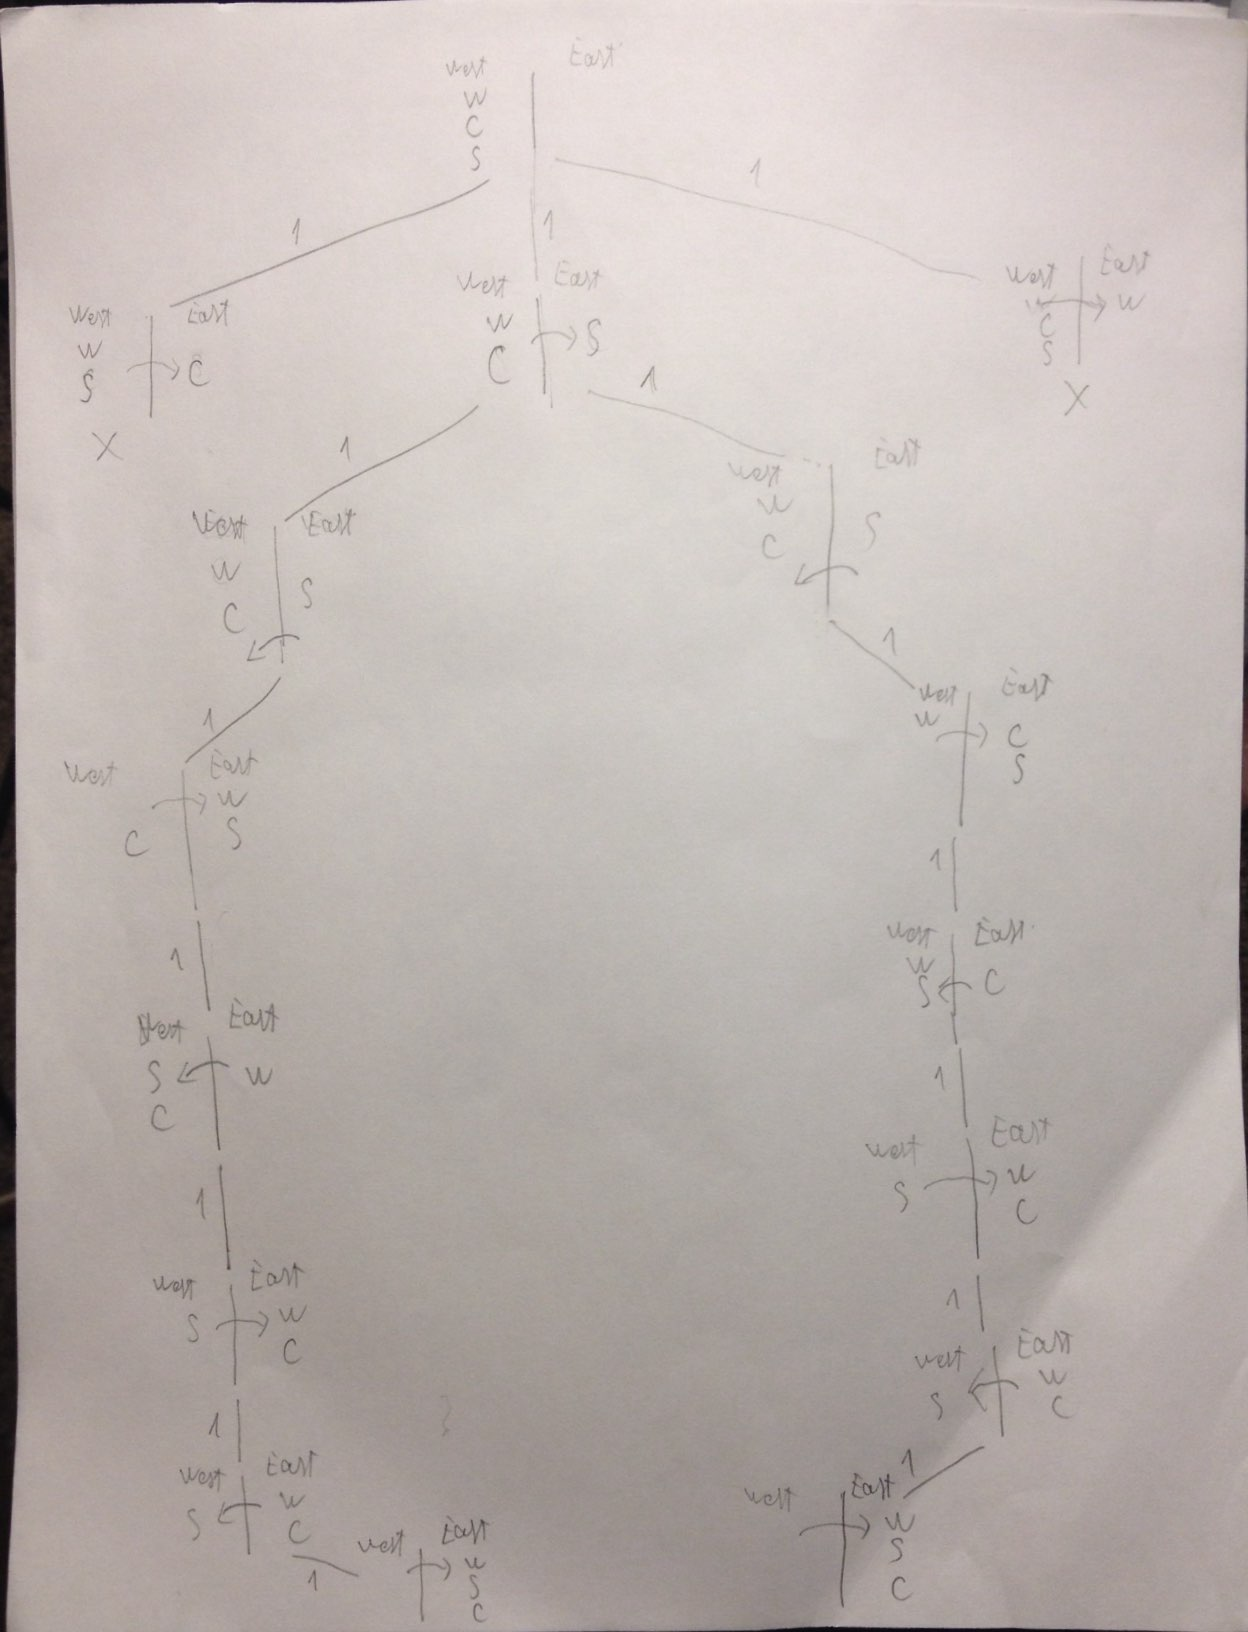
\includegraphics[scale=0.35]{problem3.jpg}
\item
There are \boxed{two} different solution (with that number of crossings)\\ 

\end{qparts}

\newpage
\section*{4. Equality contrains}
\Large{}
\noindent
\textbf{Main idea.}\\
The idea is to make the graph of all equality constraints in m constraints, the edges represent the equality relationship between two variables. After having a graph, running DFS to get all the sets of vertices that are strongly connected components. Then iterate through the inequality constraints, for 2 variables in each inequality constraint , make sure that these no strongly connected components set contains both 2 variables, if so, the constrains are satisfied. If there is a set contains both 2 variables, it means that the constrains cannot be simultaneously satisfied.\\

\noindent
\large{}
\textbf{Pseudocode.}\\
Line 0: Function(m constraints):\\
Line 1:\tab G = make a graph of all equality constraints in m constraints\\
Line 2:\tab SCCSets= run DFS on G,get the sets of vertices that are strongly connected component\\
Line 3:\tab For a and b in each pair of variables in inequality constraints in m constraints:\\
Line 4:\tab\tab For H in SSCSets:\\\
Line 5:\tab\tab\tab If (a in H) and (b in H): Output "NO" and return False\\
Line 6:\tab return True\\ 
\noindent
\Large{}
\textbf{Proof of correctness.}\\
\_ Direct proof:\\
In the m constraints, we have equality constraints and inequality constraints. In the equality constraints, an edge in graph G represent equality relationship between 2 variables. If $v_i = v_{i+1}$ and $v_{i+1} = v_{i+1}$ means that there is an edge between $v_i\ and\ v_{i+1}$, and an edge between $v_{i+1}\ and\ v_{i+2}$. We also can see that $v_i = v_{i+2}$ since there is a path from $v_i$ to $v_{i+2}$. Hence, in the inequality constraints, if there exist a path between 2 variables in equality graph, it violated the constraints. Otherwise, if no path exist between 2 variables in each inequality constraint, then all constraints are satisfied. Therefore, the algorithm does work for 
determined whether the constraints can be simultaneously satisfied.\\

\noindent
\textbf{Running time.}
$$\boxed{T(m,n) = \Theta(m + n)}$$


\noindent
\Large{}
\textbf{Justification of running time.}\\
Let T(m, n) be the run time of the algorith, with m constraints over n variables.\\
At line 1, create a graph will take $\Theta(m)$\\
At line 2, run DFS to get the sets of vertices that are strongly connected component will take $\Theta(m + n)$\\
In the loop from line 3 to line 5, iterate through the inequality constraints, checking if pair of variables in the sets of strongly connected component, they all takes $\Theta(m)$\\
Therefore, the total run time\\
$$T(m,n) = \Theta(m) + \Theta(m + n) + \Theta(m)$$
$$\boxed{T(m,n) = \Theta(m + n)}$$

\newpage
\section*{5. Telephone keypad entry}
\noindent
\Large{}
\textbf{Main idea.}
The idea is to find probability of every vertex in the graph. Reverse all the edges of the graph. Start from the sink node t, find the child node that has maximum probability among node t's children, and add it to the list of words. Then, start from the child node which has the maximum probability  among node t's children, find the child node that has maximum probability among that node's children, and add it to the list of words. Keep going until it hit the source node s. Now, we have a list of words, reverse it and return the reverse list of words.\\
How to calculate the probability of vertex.\\
As the example in the homework
$$P(me,S) = P(me, hive, S) + P(me, give, S)$$
$$P(me|hive) P(hive) = P(me,hive) = P(me,hive,S)$$
$$P(me|give) P(give) = P(me,give) = P(me,give,S)$$
\noindent
\textbf{Pseudocode.}\\
\large{}
Line 0: words = []\\
Line 1: JointWords(graph G):\\
Line 2:\tab dict = empty dictionary (key: vertex, values: P(vertex, s) )\\
Line 3:\tab For v in V in graph G:\\
Line 4:\tab\tab sum = 0 (this is P(v,s))\\
Line 5:\tab\tab for each vertex z that point to v:\\
Line 6:\tab\tab\tab sum = sum + $P(z|v) \times P(z)$\\
Line 7:\tab\tab dict[v] = sum\\
Line 8:\tab G = reverse all the edges\\
Line 9:\tab v = t, sink node\\
Line 10:\tab While(v is not s, source node):\\
Line 11:\tab\tab get the maximum probability in dicts of a child node in children of v and add it to list words, and set v to that maximum probability child\\
Line 12:\tab words = reverse(words)\\ 
Line 13:\tab return words\\

\Large{}
\noindent
\textbf{Proof of correctness.}\\
\_ Direct proof:\\
We know that after find all the probability. Reverse all the edges and find the words from the sink node t travel all the way to the source node s. Let say we start from node t, and we find a node $W_k$  that has the maximum probability $P(t|W_k)$ among t's children. And then we do the same thing for node $W_k$ that has the maximum probability $P(W_{k-1}|W_k)$ among  $W_k$'s children. Hence, we will have a collection of all the maximum probability that their product also the maximize $P(W_k|W_{k-1}) \cdots P(W_3|W_2)P(W_2|W_1)P(W_1|W_0)$. At the end we just return the list of the words correspond to these maximum probability. Therefore, the algorithm is work to find The sequence of words $w1, w2, \cdots   ,wk$ that maximize $P(W_k|W_{k-1}) \cdots P(W_3|W_2)P(W_2|W_1)P(W_1|W_0)$, out of all possible decodings consistent with the graph

\noindent
\textbf{Running time.}
$$\boxed{T(E,V) = \Theta(|E| + |V|)}$$

\noindent
\textbf{Justification of running time.}
Let T(E,V) be the run time of the algorithm, with E edges and V vertices.\\
Compute the probability for each vertex require iterate through the vertices and go through all the edges which take $\Theta(|E| + |V|)$.\\
Reverse all the edges take $\Theta(|E| + |V|)$.\\
Going backward from the sink to the source node take $\Theta(|E| + |V|)$\\
Therefore, 
$$T(E,V) = \Theta(|E| + |V|) + \Theta(|E| + |V|) + \Theta(|E| + |V|)$$
$$\boxed{T(E,V) = \Theta(|E| + |V|)}$$
\end{document}
